%======================================================================
\subsection{BW-SIM-01 modal and buckling --- Built, 30 Oct: modes, load factors, prestress, nonlinear buckling, playback}\label{sec:sim-modal-built}
%======================================================================

Modal frequencies and structural buckling now run on the static frame of \S\ref{sec:sim01-built}, built on your
answers of 30~Oct (\S\ref{sec:sim-modal-plan}, M1--M5 and B1--B3, all ``now''). The work is in seven commits:
\code{473e86c9} (modal, and the headless module \file{src/Mod/BruceWorx/bruceworx\_sim\_eigen.py} with all four
paths), \code{a4e4819a} (buckling), \code{13fda65e} (prestressed modal), \code{9938ebae} (nonlinear buckling),
\code{9d326390} (New Study finds a part an earlier study already meshes), \code{b15548e4} (the panels, mode playback
and the Motion Study timeline) and \code{31d0c682} (a FreeCAD colouring bug found on the way). The static-study
follow-ups you approved the same day are at the end (\S\ref{sec:sim-static-followups}).

\begin{figure}[!htbp]
\centering
\begin{minipage}[b]{0.6\linewidth}\centering
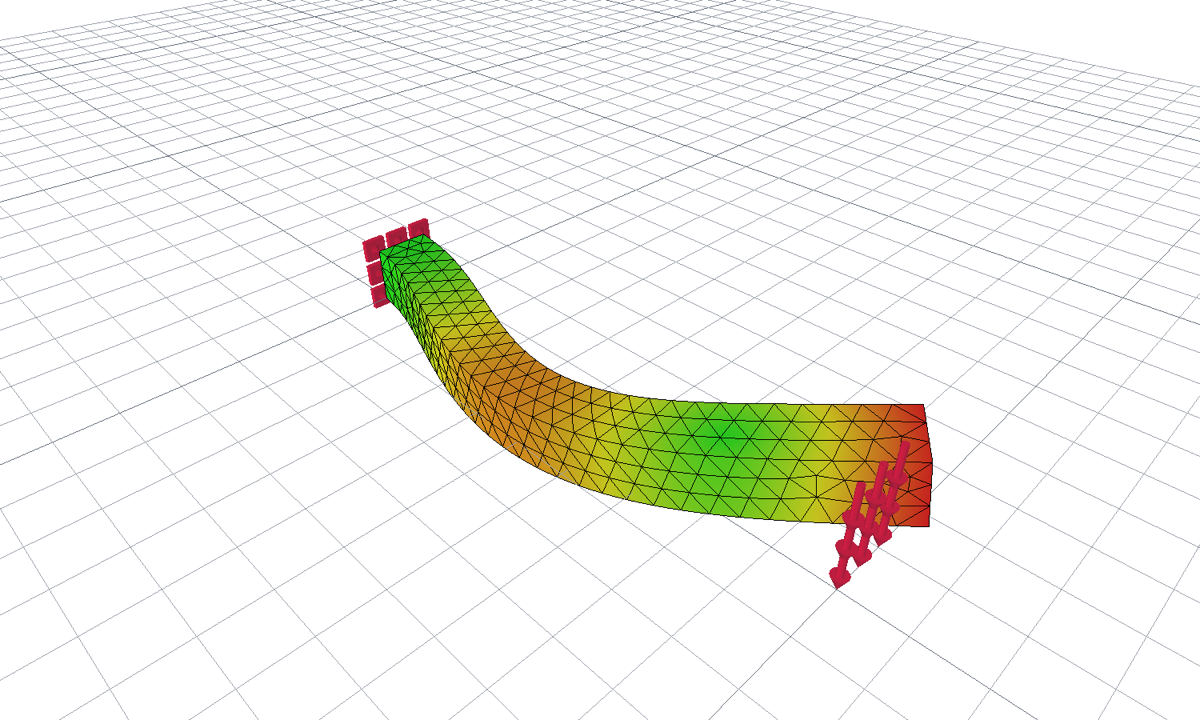
\includegraphics[width=\linewidth]{fig/simmodal_mode3.png}\\[2pt]
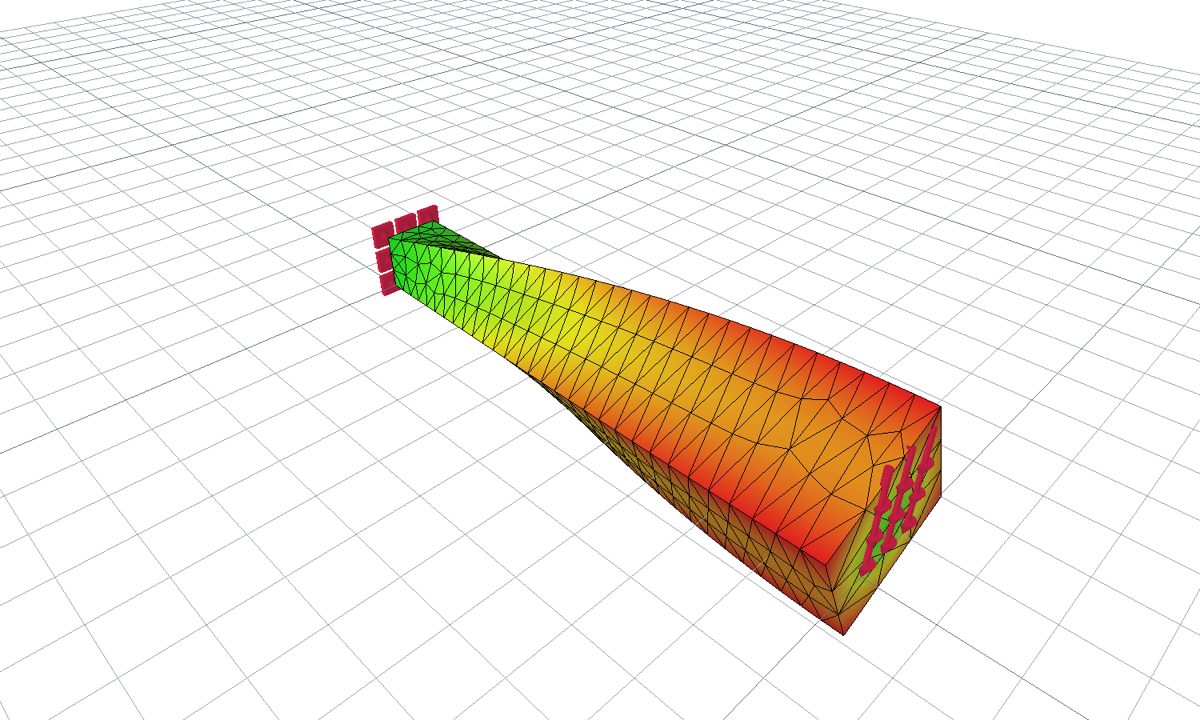
\includegraphics[width=\linewidth]{fig/simmodal_mode5.png}
\end{minipage}\hfill
\begin{minipage}[b]{0.37\linewidth}\centering
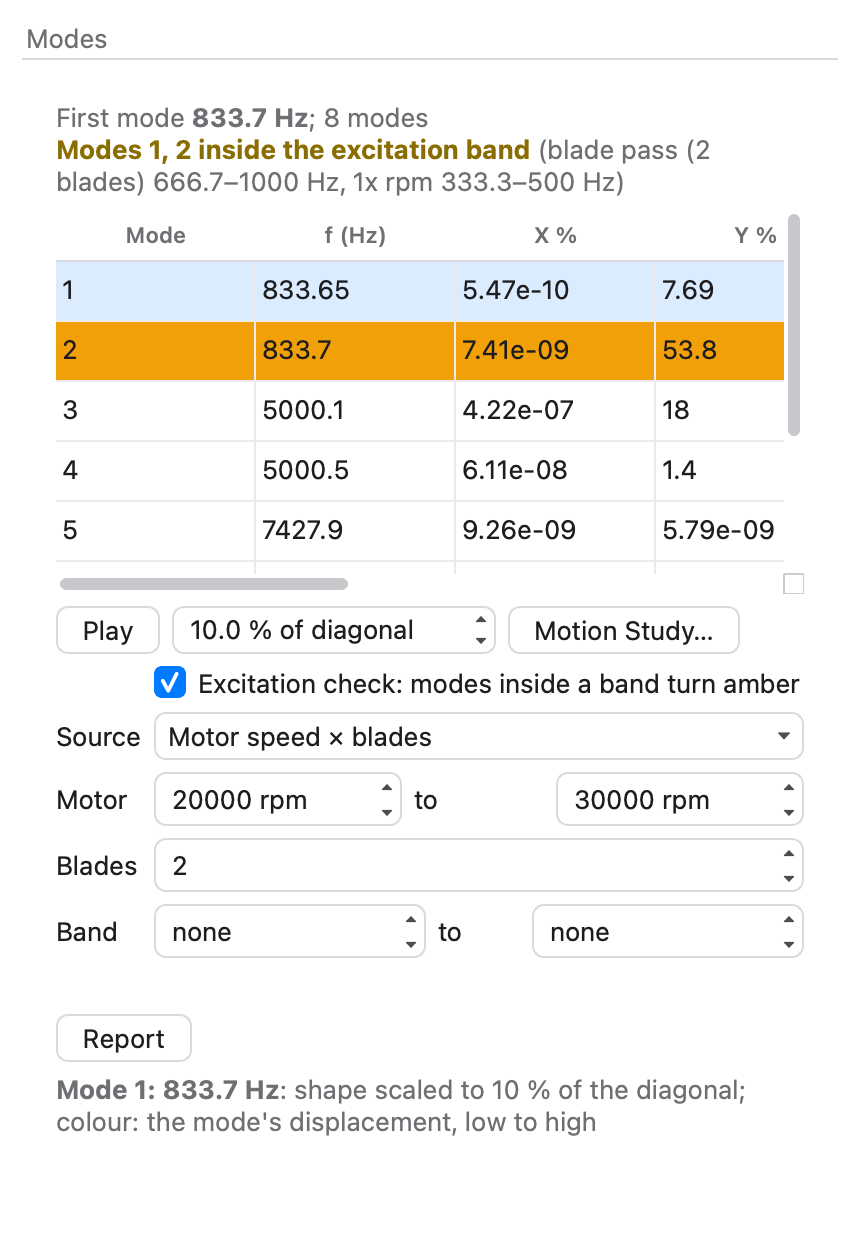
\includegraphics[width=\linewidth]{fig/simmodal_panel.png}
\end{minipage}
\caption{The cantilever benchmark ($100\times10\times10$\,mm steel, fixed at the left) as a modal study. Left:
mode~3, the second bending mode (5000\,Hz), and mode~5, torsion (7428\,Hz), each scaled so its largest
displacement is 15\,\% of the bounding-box diagonal and coloured by the mode's displacement. Right: the study
panel's Modes box with the excitation check on (20\,000--30\,000\,rpm, 2~blades: blade pass 667--1000\,Hz):
modes 1 and 2 at 833.7\,Hz are inside the band and turn amber (row~1 shows the selection colour). The
tip-load arrows belong to the static study's load, which a plain modal study ignores. Off-screen renders of the
real objects.}
\label{fig:simmodal-modes}
\end{figure}

\paragraph{What you can do now.}
\begin{itemize}[nosep]
  \item \textbf{New Study} lists Modal frequencies and Structural buckling as available (Thermal and Thermal stress
        stay planned). Modal asks for the modes (8), an optional range ($f_{\min}$--$f_{\max}$, ``none'' by
        default) and \emph{Prestressed}; buckling for the load factors (4), the target factor (3) and
        \emph{Nonlinear}. The stress-measure row shows for static studies only.
  \item \textbf{The pre-check} by type. Modal: the material needs a density; no supports is a warning (free-free:
        the six rigid-body modes are asked for on top of the count, skipped in the table and reported); loads
        are a warning (ignored) unless the study is prestressed, which needs supports and a load like a static
        one. Buckling: supports and a load (``the reference load'') are required. The strength warnings are for
        static studies only.
  \item \textbf{The study panel} keeps Setup, Mesh and Solve; the Solve box carries the type's settings (they apply
        at the next solve) and the Results box becomes a mode table. Modal: mode, $f$, effective modal mass in
        X, Y, Z (\%); the excitation editor (on/off, motor rpm range $\times$ blades or a plain band); excited
        modes amber, and a summary line naming them and the bands (blade pass and 1$\times$\,rpm). Buckling:
        mode, $\lambda$, a ``$\lambda_1$'' or ``reversed load'' note, $\lambda$ coloured red below 1, amber below the
        target, green at or above it; the target can be changed and saved as the default; the summary carries
        the non-conservative line and, after a nonlinear run, its collapse factor.
  \item \textbf{Mode shapes}: a row shows its mode on the result mesh at 10\,\% of the bounding-box diagonal (the
        study's \code{ModeScale}, settable as ``\% of diagonal''); \emph{Play} animates
        $\mathbf u=s\boldsymbol\phi\sin2\pi t$ at one cycle per second by moving the mesh nodes (a timer and
        \code{applyDisplacement}, as the static deformed view does). \emph{Mode Shapes} on the Results ribbon opens
        the panel playing.
  \item \textbf{Motion Study} (M2): \emph{Motion Study\ldots} in the panel, or the ribbon's Motion Study command with a
        mode result selected, puts the mode on the Motion Study timeline: cycles, seconds per cycle and frame rate,
        then the same scrub slider, $|\!<$ $<$ Play Stop $>$ $>\!|$, Once/Loop/Ping-pong, speed and \emph{Save
        frames} (PNG frames and \file{motion.mp4} with ffmpeg) as an assembly's motion study. Closing it returns
        to the study panel.
  \item \textbf{The report} by type. Modal: the frequency table with the modal mass and the excited modes boxed in
        amber, the rigid modes left out, the range, the prestress line, the excitation section (the bands and the
        verdict), renders of the mesh and the first three modes. Buckling: the load-factor table coloured against
        the target, the $\lambda_1$ verdict, the boxed non-conservative note, renders of the first two buckled shapes
        (positive factors first), and for a nonlinear run its description, the collapse factor and a pgfplots
        curve that Tectonic draws.
\end{itemize}

\begin{figure}[!htbp]
\centering
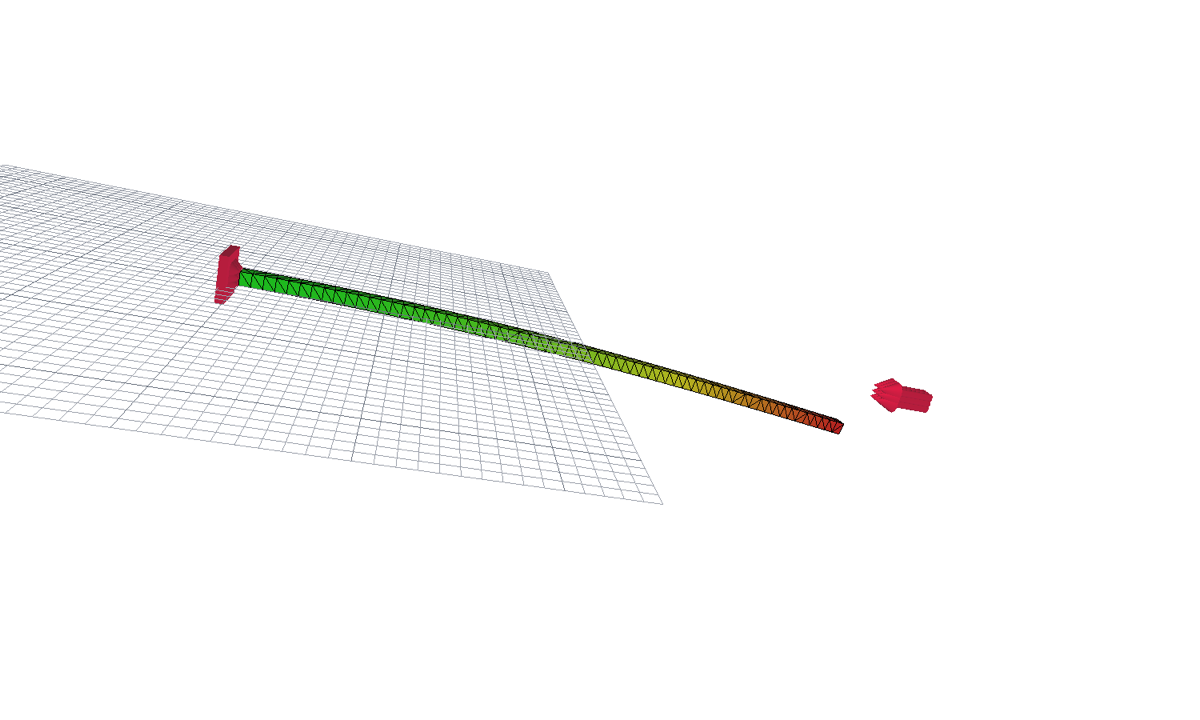
\includegraphics[width=0.49\linewidth]{fig/simmodal_buckle1.png}\hfill
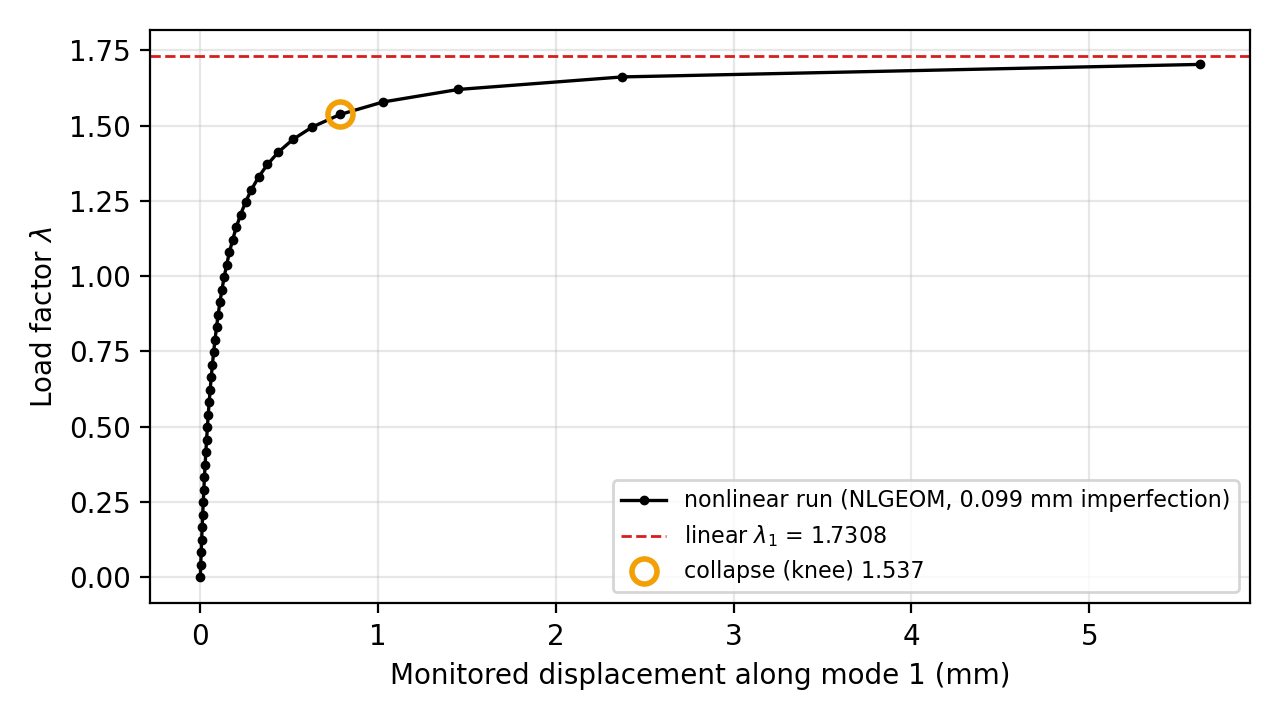
\includegraphics[width=0.49\linewidth]{fig/simmodal_curve.png}
\caption{The Euler column ($500\times10\times10$\,mm steel, clamped, 1000\,N towards the clamp). Left: buckled
shape~1 ($\lambda_1=1.7308$), scaled to 12\,\% of the diagonal; the load arrow stays at the undeformed tip.
Right: the nonlinear run with a 0.099\,mm imperfection along mode~1 (1\,\% of the section): load factor against
the tip's displacement along mode~1. The curve bends over towards $\lambda_1$ and the knee (slope below 1\,\% of
its start) is at 1.537, 89\,\% of $\lambda_1$; past 1.703 the run jumped to the other side and is cut
(\emph{Decided while building}). The report draws the same curve with pgfplots.}
\label{fig:simmodal-buckling}
\end{figure}

\paragraph{Benchmarks} (\eref{SIM-05}, in \file{TestBruceWorxSimCore}; the solver tests skip without \code{ccx}).
\begin{center}
\small\setlength{\tabcolsep}{4pt}
\begin{tabular}{@{}llll@{}}
\toprule
Case & FE & Reference & Error\\
\midrule
Cantilever $f_1$ (a pair) & 833.65, 833.70\,Hz & 835.5\,Hz (E--B) & $-0.2$\,\%\\
Cantilever $f_2$ (a pair) & 5000.1, 5000.5\,Hz & 5236 E--B, 5051 Tim. & $-4.5$ / $-1.0$\,\%\\
Cantilever $f_3$ (a pair) & 13167.6, 13169.4\,Hz & 14661 E--B, 13335 Tim. & $-10.2$ / $-1.3$\,\%\\
Cantilever, torsion; axial & 7427.9; 12972\,Hz & axial: 81\,\% X mass & \\
Free-free bar $200\times10\times10$ & 6 rigid, then 1317.5\,Hz & 1329.1\,Hz ($\beta L=4.7300$) & $-0.9$\,\%\\
Tensioned beam, $T=10$\,kN, $f_1$ & 146.60 (146.89)\,Hz & 146.76\,Hz & $-0.1$\,\%\\
\quad the same, $f_2$ & 433.6\,Hz & 437.9\,Hz & $-1.0$\,\%\\
\quad the same beam unloaded & 93.57\,Hz & 93.81\,Hz & $-0.3$\,\%\\
Euler column $\lambda_1$ (8\,mm mesh) & 1.7308 (1.7319) & 1.7272 & $+0.2$\,\%\\
Euler column $\lambda_2/\lambda_1$, same plane & 8.981 & 9 & $-0.2$\,\%\\
Column, load reversed & four negative factors & no positive one & \\
Nonlinear column, $e_0=0.099$\,mm & collapse 1.537 & below $\lambda_1$ & $0.888\,\lambda_1$\\
\bottomrule
\end{tabular}
\end{center}
The plan's ``$f_1\approx837$\,Hz'' is 835.5\,Hz with $\beta_1L=1.8751$. The cantilever has $L/h=10$: from the second mode on it is a Timoshenko beam, so $f_2$ and $f_3$ lie 4.5 and
10\,\% below Euler--Bernoulli, outside the $\pm3$ and $\pm8$\,\% the plan set against 5.25 and 14.7\,kHz. The test
checks $f_1$ against Euler--Bernoulli ($\pm3$\,\%) and $f_2$, $f_3$ against the Timoshenko values ($\pm3$ and
$\pm8$\,\%; they agree to 1.0 and 1.3\,\%), which use the Rayleigh--Timoshenko first-order correction
$f_T=f_{EB}/\sqrt{1+(\beta r)^2(1+E/\kappa G)}$ with Cowper's $\kappa$ (question~1). The free-free bar was made
200\,mm long ($L/h=20$) so that Euler--Bernoulli's 4.7300 applies. The prestressed benchmark uses
$f_1=\frac{1}{2L}\sqrt{T/\rho A+EI\pi^2/(\rho AL^2)}$: the brief's $\pi/2L$ in front is a typo, it would be
$\omega/2$.

\paragraph{Decided while building.}
\begin{itemize}[nosep]
  \item \textbf{Effective modal mass from the .dat.} CalculiX 2.23 writes, for every \code{*FREQUENCY} step, the
        eigenvalue table, the participation factors, the effective modal mass per mode (X, Y, Z and three
        rotations) and the total effective mass. The table shows the mode's mass in X, Y and Z as a share of the
        total effective mass (the mass that can move: on the cantilever 78.0 of 78.5\,g, the fixed face's nodes
        excluded). Frequencies and ccx mode numbers also come from the .dat: CalculiX drops a rigid mode whose
        eigenvalue comes out slightly negative, so its numbering starts above 1, and FreeCAD's own .dat match
        then gives every free-free mode the wrong frequency. The study writes the right value back into
        \code{EigenmodeFrequency}.
  \item \textbf{Buckled shapes are read by the study.} FreeCAD's FRD import starts a new result only when the step
        value rises, so two equal factors (a square column's pair) or negative ones merge into one result. The
        study reads the .frd's displacement blocks itself (fixed columns: a negative factor runs into the set
        number, ``\code{102-1.24311E+05}'') and makes one result per mode; the first set is the reference state
        and is skipped.
  \item \textbf{Prestressed modal is \code{*STEP, PERTURBATION}.} Checked in ccx 2.23: a \code{*FREQUENCY} step after
        a static step ignores the previous state unless the step has PERTURBATION; with it, a linear static step
        and an NLGEOM one give the same frequencies to 0.02\,\% on the tensioned beam, so the static step is
        linear. FreeCAD's writer writes that step as for a static study; the study adds the \code{*DENSITY} card (the
        writer writes it only for a frequency analysis) and the second step. Compressive prestress lowers the
        frequencies the same way.
  \item \textbf{Nonlinear buckling, load-controlled.} CalculiX has no Riks arc-length method (no RIKS in the 2.23
        binary). The run is the linear buckling input changed: the nodes moved by the imperfection, the loads
        times $1.2\,\lambda_1$ (\code{NonlinearLoadLimit}), \code{*STEP, NLGEOM} with automatic \code{*STATIC} increments
        (2\,\% of the load at most) and the monitored node printed every increment. Prescribed displacements are not
        scaled.
  \item \textbf{The imperfection amplitude}, when not set: 1\,\% of the smallest section dimension, taken as the
        smaller of the bounding box's shortest edge and the hydraulic diameter $4V/S$. $4V/S$ is the side of a
        square bar (9.90\,mm for the column, the end faces aside), the diameter of a round one, and twice the wall
        of a thin shell, whose bounding box says nothing about its wall; a plate gets its thickness from the box.
        The report says which.
  \item \textbf{The collapse load factor} is the knee: the first increment after which the curve's slope falls below
        1\,\% of its initial slope; else, when the run stops converging, its last converged increment (a limit
        point, as a thin shell would have). For an imperfect strut $u=e_0/(1-\lambda/\lambda_{cr})$ the 1\,\% knee
        is at $0.9\,\lambda_{cr}$, which is where the column landed. The monitored displacement is the node where
        $\boldsymbol\psi_1$ peaks, along $\boldsymbol\psi_1$.
  \item \textbf{The curve is cut where the run leaves the path.} Under load control the near-perfect column jumped
        to the other side just past $\lambda_1$ (from $+5.6$ to $-12.4$\,mm in one increment) and then converged
        back towards the straight, unstable state as the load rose. Increments where the monitored displacement
        changes sign or shrinks while the load grows are not a load path; the curve stops before them and the
        report says so. A finer mesh (5\,mm) and 1.5\,$\lambda_1$ ran smoothly to 390\,mm in a hand test.
  \item \textbf{Free-free asks for six more modes.} With no supports and no range above 1\,Hz the solver is asked
        for \code{ModeCount}\,$+\,6$, so the table still has eight elastic modes.
  \item \textbf{The timeline, shared (M2).} The Motion Study timeline of ROB-05 drives an assembly through the
        kinematic solver (\code{generateSimulation}, \code{updateForFrame}); a mode shape is a mesh deformation the
        solver cannot carry, so a mode does not become a joint channel. Instead the timeline itself is now
        \code{TimelineMixin} in \file{bruceworx\_motion.py} (scrub, transport, loop modes, speed, Save frames), which
        \code{MotionStudyPanel} uses unchanged and a mode plays on as another frame source; \code{save\_frames} takes
        a \code{show(index)} for it, and the Motion Study command opens a selected mode through
        \code{register\_source}, so motion knows nothing about simulation. The ROB-05 tests pass as before.
  \item \textbf{Fixed on the way:} New Study found no part once a study existed (the mesh takes the part as a child,
        so it leaves the root objects; \code{9d326390}).
\end{itemize}

\paragraph{Tests.} Headless (\file{TestBruceWorxSimCore}, 40 in 11\,s): the .dat and .frd readers on fixed samples, the
input changes (density, perturbation step, scaled loads, moved nodes, the nonlinear step), the collapse point and
the cut curve, the colour status and the bands, the theory functions; modal and buckling defaults and pre-checks,
the excitation bands, the target preference, the section size and the imperfection; then the benchmarks of the
table, the reports' sources, and the nonlinear report compiled with Tectonic. GUI (\file{TestBruceWorxSimulation},
10 in 14\,s): New Study for both types; a modal solve with the table, a row shown, the scale, play and pause, the
excitation colours, the timeline (50 frames by default, 10 at 5\,fps, ping-pong, ten PNGs saved), the Motion Study
command on a selected mode, and a report with four figures compiled; a buckling solve with the nonlinear run, the
colours, a target of 1.5 turning $\lambda_1$ green and saved as the default, and a report with two figures and the
pgfplots curve. \file{TestBruceWorxMotion} (16; one Drive Joint animation test is timing-sensitive and failed once
under load, then passed), \file{TestBruceWorxWorkspaces} (25), the connection lint in \file{TestBruceWorx} (15) and
\file{AssemblyTests.TestBWMotion} (16) pass.

%----------------------------------------------------------------------
\subsubsection*{Static follow-ups (30 Oct)}\label{sec:sim-static-followups}
%----------------------------------------------------------------------

Your answers to the five open questions of \S\ref{sec:sim01-built}, built after the modal and buckling work.

\begin{figure}[!htbp]
\centering
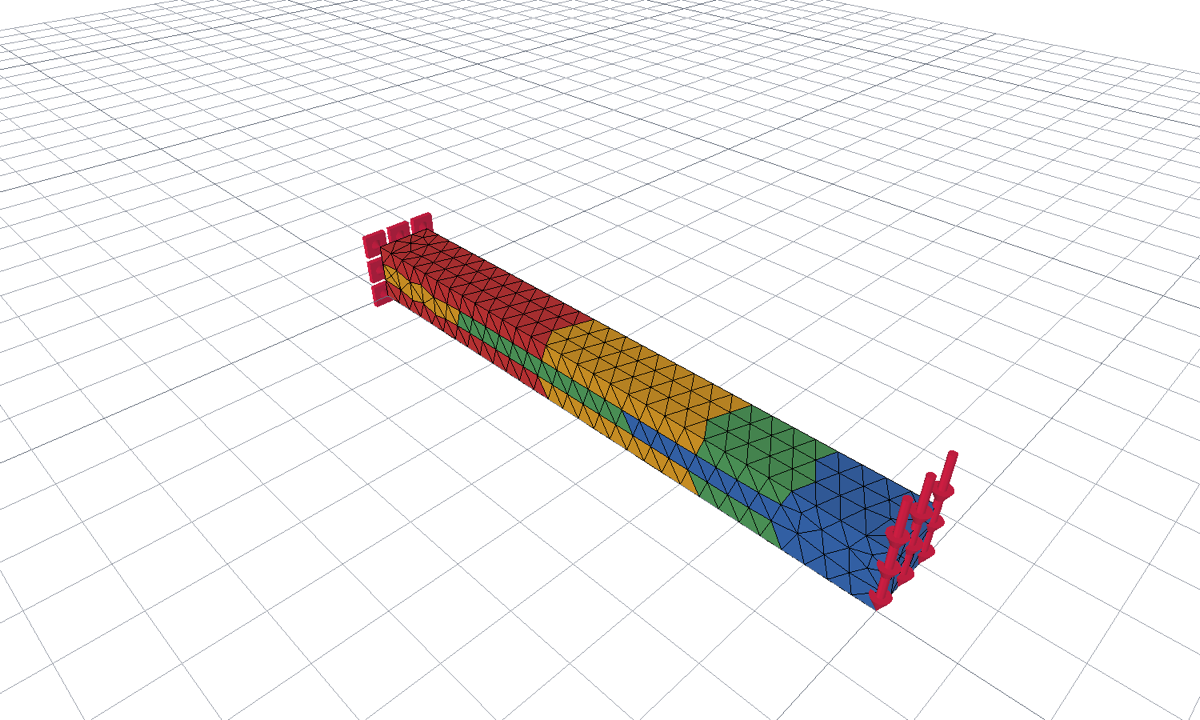
\includegraphics[width=0.62\linewidth]{fig/simmodal_sfbands.png}
\caption{The static cantilever in four safety-factor bands, now crisp: each element in the band of its lowest node
(red below 1 at the root's top and bottom fibres, then amber, green, and blue towards the free end). Compare
Fig.~\ref{fig:sim01-built}, which blurred each band edge across one element.}
\label{fig:simmodal-sfbands}
\end{figure}

\begin{enumerate}[nosep]
  \item \textbf{Crisp bands} (\code{dc5fcf4d}, \code{31d0c682}). The safety-factor view colours each element by its
        lowest node's safety factor (\code{ElementColor}, colour mode ByElement); the band edges are element edges.
        Stress and displacement stay smooth, and so do the mode shapes (they have no bands). The first renders were
        a random patchwork: FreeCAD's \code{ViewProviderFemMesh} draws a 6-node face as four triangles but recorded
        the element of only three, so every colour after the first quadratic face was off by one triangle per face.
        33 lines in that file give every inner triangle (6- and 8-node faces of every element type) its entry.
  \item \textbf{Singularities at fixed faces} (\code{dc5fcf4d}). The result carries \code{SupportNodes}, the nodes on
        the supports (from the study's mesh, matched to the result mesh by position), and
        \code{MinSafetyFactorAwayFromSupports}. The panel and the report give both minima with one line: a fully
        fixed face cannot contract sideways, so its edges are a singularity that grows with refinement. On the
        cantilever (27 nodes on the face) von Mises gives 0.574 either way (its peak is just off the face) and
        Rankine 0.435 on the face, 0.544 away from it.
  \item \textbf{Tectonic offline} (\code{52823a9d}). \file{make-keystone.sh} compiles
        \file{tectonic-seed/seed.tex} (beside the script) once with \code{TECTONIC\_CACHE\_DIR} in
        \file{Contents/Resources/tectonic-cache} (about 16\,MB, network needed at bundle time), then again with
        \code{-{}-only-cached} to prove it complete; a failure leaves no seed and a warning. At run time the seed is
        copied once into \file{\textasciitilde/Library/Caches/Keystone/tectonic} (the bundle stays read-only) and
        Tectonic is pointed there. The seed document loads every package the reports use and prints every size and
        shape they do: the first seed missed 9\,pt typewriter and 6\,pt math italic, found by compiling the five
        report kinds with \code{-{}-only-cached}, which all pass now. A test keeps the seed's packages a superset of the
        reports'. Not run here: a full bundle build (the main session stages Keystone).
  \item \textbf{The report in the vault: a gap.} Check-in (\code{FolderVault.checkin}) stores one file per version and
        has no attachments; attachments exist only on lifecycle records (approve, reject, ECR, ECO release). Nothing
        was invented: attaching the study PDF needs either an \code{attachments} field on the check-in event (PDM
        schema, \file{addons/BruceWorx/bruceworx/pdm\_folder.py}, which another session is editing) or the newest
        report offered as an attachment at Approve and Release ECO (question~5).
  \item \textbf{Preferences} (\code{547f1488}). Preferences $\cdot$ BruceWorx $\cdot$ Simulation: band edges and colours
        (refused with the reason when they do not rise), stress measure, modal modes and buckling factors, target
        buckling load factor, mesh divisor (the default element size is the diagonal over it) and the TeX compiler,
        all in \code{Mod/BruceWorx/Sim}; New Study and new studies read them.
\end{enumerate}

\paragraph{Open questions for you.}
\begin{enumerate}[nosep]
  \item \textbf{The cantilever's $f_2$ and $f_3$.} On the $100\times10\times10$ bar they are 4.5 and 10\,\% below the
        Euler--Bernoulli values of the plan, as a Timoshenko beam should be; the test checks them against the
        Timoshenko values. Keep that, or move the higher-mode check to a slender bar (e.g.\ $300\times10\times10$) where
        Euler--Bernoulli holds?
  \item \textbf{The knee criterion.} The nonlinear collapse factor is where the slope falls below 1\,\% of its start
        ($0.9\,\lambda_{cr}$ for an imperfect strut). A stricter 0.1\,\% would put it at $0.97\,\lambda_{cr}$; Fusion
        reports no such point. Keep 1\,\%, or report the load at a displacement limit you set?
  \item \textbf{Default load limit} for the nonlinear run: $1.2\,\lambda_1$ keeps it short (12\,s on the column) but
        ends before a stable post-buckling path is seen. Raise it for plates and shells, whose post-buckling
        strength is real?
  \item \textbf{Excitation harmonics.} The motor check uses the blade-pass and 1$\times$\,rpm bands. Add 2$\times$ blade
        pass (and an ESC PWM line) for the drone, or keep two bands?
  \item \textbf{The study PDF in the vault} (follow-up 4): an \code{attachments} field on check-in, or the newest report
        attached at Approve and Release ECO? Either is a PDM change; which session should make it?
\end{enumerate}

\paragraph{Answers (30 Oct).}
\begin{enumerate}[nosep]
  \item \textbf{Higher modes:} move the check to a slender bar and compare with Euler--Bernoulli
        (\code{4c6a5313}); the thick bar stays checked against Timoshenko.
  \item \textbf{Knee criterion:} report the load at an optional displacement limit you set for the nonlinear
        collapse run (\code{2d87a5a2}).
  \item \textbf{Nonlinear load limit:} a setting, default $1.5\,\lambda_1$ (\code{2d87a5a2}).
  \item \textbf{Excitation harmonics:} add the $2\times$ blade-pass band (\code{5ec45ae4}).
  \item \textbf{Study PDF in the vault:} offered as attachments at Approve and Release ECO, not on check-in.
        The panels tick the newest \code{<part number>\_<study>\_report.pdf} files beside the work copy
        (\code{bruceworx.sim\_reports}); \code{vault approve -{}-attach-reports} does the same on the command line.
        Commit: see \code{git log} subject ``SIM-01: study reports offered as attachments''.
\end{enumerate}
